% ****** Start of file aipsamp.tex ******
%
%   This file is part of the AIP files in the AIP distribution for REVTeX 4.
%   Version 4.1 of REVTeX, October 2009
%
%   Copyright (c) 2009 American Institute of Physics.
%
%   See the AIP README file for restrictions and more information.
%
% TeX'ing this file requires that you have AMS-LaTeX 2.0 installed
% as well as the rest of the prerequisites for REVTeX 4.1
% 
% It also requires running BibTeX. The commands are as follows:
%
%  1)  latex  aipsamp
%  2)  bibtex aipsamp
%  3)  latex  aipsamp
%  4)  latex  aipsamp
%
% Use this file as a source of example code for your aip document.
% Use the file aiptemplate.tex as a template for your document.
\documentclass[%
 aip,
 % onecolumn,
% jmp,
% bmf,
% sd,
 % rsi,
 amsmath,amssymb,
%preprint,%
 reprint,%
%author-year,%
%author-numerical,%
% Conference Proceedings
floatfix,
% tikz,
]{revtex4-1}

\usepackage{graphicx}% Include figure files
\usepackage[utf8]{inputenc}
\usepackage[T1]{fontenc}
\usepackage{mathptmx}
\usepackage{tikz}
\usetikzlibrary{arrows,decorations.markings,decorations.pathmorphing, patterns,shapes}
\usepackage{dcolumn}% Align table columns on decimal point
\usepackage{bm}% bold math
\usepackage{float}
%\usepackage[mathlines]{lineno}% Enable numbering of text and display math
%\linenumbers\relax % Commence numbering lines

\begin{document}
\preprint{AIP/123-QED}

\title[]{The Busch Helical Method: \\ Measuring the Ratio of an Electron's Charge to Mass}
% Force line breaks with \\

\author{Jared Baur and Ben Sappey}
 % \altaffiliation[Also at ]{Physics Department, XYZ University.}%Lines break automatically or can be forced with \\
% \author{Ben Sappey}%
% \affiliation{ 
% Authors' institution and/or address%\\This line break forced with \textbackslash\textbackslash
% }%

\date{\today}% It is always \today, today,
             %  but any date may be explicitly specified


\begin{abstract}

	Write abstract here.

\end{abstract}

\maketitle


\onecolumngrid

\section{\label{sec:level1}Objective}

	Measure the charge-to-mass ratio of the electron using the Busch Helical Method.

\section{\label{sec:level2}Introduction}

In 1922, Busch developed a method of measuring the ratio of an electron's charge to its mass. This method involved focusing a divergent beam of electrons via a magnetic field. The electrons travel through a cathode ray tube in a specific trajectory. The trajectory of an electron in the presence of a magnetic field, when the electron is not moving parallel to the field, is in a helical motion. For mathematical purposes, this helical motion can be described as traveling along the surface of a cylinder. The electrons start from a hot cathode at the base of the tube. They pass through an anode with a velocity that depends on the potential difference between the cathode and the anode. This potential difference is called the "accelerating voltage". The applied magnetic field in the solenoid cause the beam of electrons to travel in the previously mentioned helical motion, completing a certain number of loops until hitting the fluorescent screen on the end of the cathode ray tube. The result from this process is a light that is emitted from the screen that changes with size as the magnetic field is changed. The original Busch design for this experiment had auxiliary magnets strategically placed around the cathode ray tube (instead of a solenoid) in order to produce the desired magnetic field\cite{Stranathan1942}.

In order to obtain the ratio of an electron's charge to its mass, let us consider a single electron moving with velocity $v$ as it exits the anode with an angle $\theta$ to the axis of the cathode ray tube. The magnetic field will influence the electron's trajectory, however only in the motion that is perpendicular to the magentic field. Thus, the longitudinal component of the velocity, $v \cos{\theta}$ will remain constant and the perpendicular component, $v \sin{\theta}$ will vary. The electron will go through a helical motion around the axis of the tube, all while traveling down the tube at a constant velocity. It will then pass through the center axis as it completes one helical revolution. The electron's perpendicular velocity component can be expressed as

\begin{figure}[H]
		\centering
		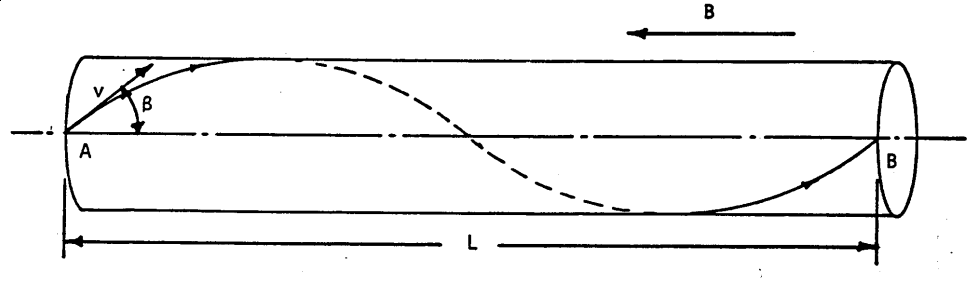
\includegraphics[scale=0.5]{electrontrajectory.png}
		\caption{Path of electrons in the solenoid. Electrons leave the cathode ray anode with a velocity $v$ at an angle $\beta$.}
	\end{figure}

\begin{equation}
	v \sin{\theta} = \frac{m(v \sin{\theta})^2}{eHR}
\end{equation}
 
\noindent where $H$ is the magnetic field, $m$ is the mass of the electron, $e$ is the charge of the electron, and $R$ is the radius of the helical path taken by the electron. The time $t$ for the electron to complete one revolution of this helix is expressed in Equation 2.

\begin{equation}
	t = \frac{2 \pi m}{H e}
\end{equation}

\noindent Solving for $R$ in either of these equations and plugging into the other will give a simplified form for the time $t$ of one revolution.

\begin{equation}
	t = \frac{2 \pi m}{H e}
\end{equation}

\noindent Since Equation 3 is independent of the perpendicular velocity, all electrons, regardless of longitudinal velocity, will complete one revolution in the same amount of time. If all electrons sent through the cathode have the same velocity (influenced by the accelerating voltage), then they will hit the fluorescent screen at the same time, thus creating a focused image on the screen. The time for the electrons to travel from the anode to the screen is expressed in Equation 4. In this equation, $L$ is the distance from the anode to the fluorescent screen.

\begin{equation}
	t = \frac{L}{v \cos{\theta}}
\end{equation}

\noindent When the magnetic field is adjusted so that there is a focused point on the screen, the time for the electron to reach the screen and the time for it to complete one revolution are equal. Thus, Equation 3 and 4 can be set equal to one another. Solving for the ratio $e/m$ gives equation 5. The velocity of the electron can be found by analyzing the kinetic energy $V e = 1/2 m v^2$, where $V$ is the accelerating voltage.

\begin{equation}
	\frac{e}{m} = \frac{8 \pi V \cos^2{\theta}}{H^2 L^2}
\end{equation}



\section{\label{sec:level3}Apparatus and Methods}

The apparatus consists of a cathode ray tube and a solenoid. The cathode ray anode emits electrons with the assistance of a high voltage power supply (Kepco Model Power Supply). The cathode ray tube is placed in the center of the solenoid with the axes of the tube and solenoid aligned. An accelerating voltage is applied to the cathode ray tube that accelerates electrons in a beam. A voltage applied to the intensity control grid by a separate power supply (Heathkit Regulated Power Supply Model PS-4) reduces the current of the emitted electron beam. The solenoid's magnetic field provides a curved, helical path for the electron beam to follow in the cathode tube. The solenoid's current is reversible via a homemade switch; when reversed, the magnetic field is reversed and the helical orientation of the electron beam is flipped (clockwise or counterclockwise).

	\begin{figure}[H]
		\centering
		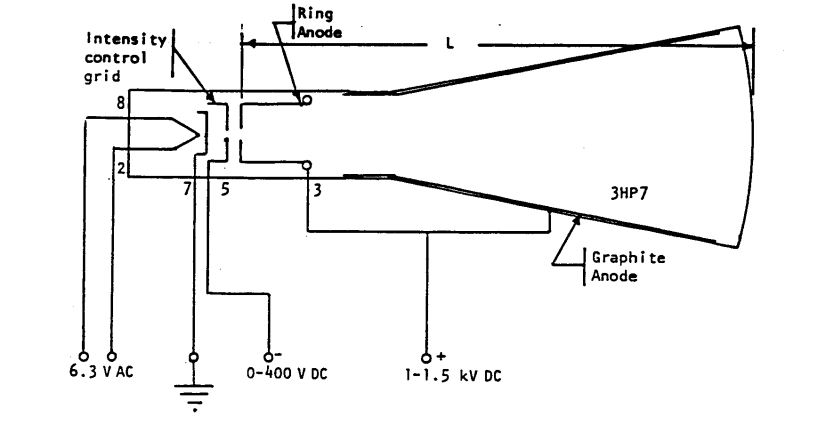
\includegraphics[scale=0.5]{cathoderaytube.png}
		\caption{Cathode ray tube schematic. Electrons are emitted from the anode and travel a distance $L$ through the cathode tube.}
	\end{figure}
Before beginning the experiment, measurements of the apparatus were made in order to obtain the values needed for calculations. The cathode ray's length $L$ was measured (used in Equation 5) with the use of a cathetometer. The cathetometer was chosen to make this measurement since it can easily be used to measure distances of objects where the measuring tool cannot be placed close to the point of interest. The cathetometer was used to measure the distance from the anode to the end of the tube (length $L$ shown in Figure 2). This length is defined as the distance from the anode to the phosphor screen that is the point at which the electrons are illuminated in the cathode tube. The phosphor screen is actually embedded underneath a glass of measurable thickness, which also required the use of a cathetometer to measure. In order to measure the glass thickness, the pinpoint of a thumbtack was placed on the surface of the glass. The microscope on the cathetometer was focused on this pinpoint and the reading on the cathetometer scale was taken. Next, the focus of the microscope was adjusted to the phosphor screen under the glass. Once the phosphor was in focus, the cathetometer scale reading was noted. The difference between these two readings represent the thickness of the glass, which was then used to calculate the actual length $L$ of the cathode ray tube (from the anode to the phosphor screen).

The magnetic field in a solenoid is given by Equation 6, where $H$ is the magnitude of the magnetic field, $n$ is the density of turns for the length of the solenoid (number of turns per unit length), $I$ is the current, and $\theta$ is the angle subtended at the center of the solenoid by the outer edge of the solenoid and its axis\cite{oxymanual}. The turn density was measured by counting the number of turns for a select unit of length, then extrapolating this small turn density to the total length of the solenoid. The angle $\theta$ was found by measuring the angle from the end of the solenoid (on the axis through its center) to the middle of the solenoid (on the solenoid's edge). The orientation of the solenoid was determined based on the earth's magnetic field. If the solenoid is placed perpendicularly to earth's magnetic field, then there would be no interference from earth's magnetic field on the electron beam. This effect is seen in the Lorentz force: $\bold{F} = q\bold{v} \times \bold{B}$; since the tangential velocity vector of the electron beam is parallel to earth's magnetic field when the solenoid is perpendicular to it, there is no outside interference. A magnetic compass was used to place the solenoid in its correct orientation.

\begin{equation}
	H = nI\cos{\theta}
\end{equation}

Before applying an accelerating voltage to the cathode ray tube, the intensity control power supply was turned on to about 300 volts. This prevented any future damage to the phosphor screen. Subsequent damage would reduce the phosphor's ability to illuminate the electron beam upon contact with the screen. Next, the accelerating voltage was applied to the cathode ray tube by turning on the main power supply to about 600 volts. A multimeter (Fluke Model 77 IV) was used to measure this voltage. Steps of about 75 volts were taken to vary the accelerating voltage throughout this experiment. The main power supply outputs its readings as kilovolts, so a volt box (Leeds \& Northup Co. Model 7593) was used to create a multiplier to convert kilovolts to centivolts (multiplier of 10,000). This allowed for a more accurate reading from the multimeter since larger values were output to the multimeter, thus allowing for the tens and ones place to be measured more accurately (since they are now visible on the multimeter screen). A current $I$ was sent down the solenoid with another power supply (Lambda Regulated Power Supply Model LR 344A FM), which was varied based on the focus of the elecron beam on the phosphor screen. For low voltage values, scanning the magnetic field through its entire range given by the current $I$, the elecron beam makes many turns in the cathode ray tube. This is seen experimentally by the focus of the beam on the phosphor screen increasing and decreasing as it travels in a circular path. The number of turns of the electron beam was reduced to one for each trial by finding the lowest possible current for which the electron beam was at focus on the phosphor screen.

For each step in the accelerating voltage, the optimal focus point of the electron beam was found, and the corresponding current from the solenoid's power supply was recorded. This current was measured with the help of a Biddle-Gray standard resistor that provides a resistance to the voltage provided from the power supply. By having this fixed resistance, the current is measured using Ohm's Law $I=V/R$. A switch is used to change the input to the multimeter from the accelerating voltage power supply to the solenoid power supply.

\section{\label{sec:level4}Data Analysis}

\section{\label{sec:level5}Conclusion}

\nocite{*}
\bibliography{main}% Produces the bibliography via BibTeX.
\end{document}
%
% ****** End of file aipsamp.tex ******
